\chapter{Construction d'un détecteur optimal}

On présente ici le détail du problème de la détection optimale quantique avec le critère de l'information mutuelle. 

\section{Formulation du problème}
Le problème de la détection d'état quantique porte sur un ensemble de $m$ états quantiques représentés par les opérateurs densité $\{\rho_i \; , \; 1 \leq i \leq m\}$ munis des probabilités à priori $\{p_i \geq 0 \; , \; 1 \leq i \leq m \}$. L'objectif est d'obtenir un ensemble de $m$ opérateurs de mesure $\{\Pi_j \; , \; 1 \leq i \leq m\}$ permettant de mesurer le mieux possible par rapport aux probabilités les états d'entrée qui nous arrivent.

Les opérateurs $\rho_i$ et $\Pi_i$ sont des matrices Hermitiennes semi-définies positives, de la forme $\begin{bmatrix}a & b+ic \\ b-ic & d \end{bmatrix}$.

Plusieurs critères ont été proposés à optimiser afin de construire ces détecteurs optimaux. D'une part, on a la possibilité de travailler sur la minimisation de l'erreur quadratique de mesure \cite{Eldar01} ou la maximisation de la probabilité de détection correcte \cite{Eldar03c}. D'autre part, et c'est ce sur quoi nous avons travaillé, on peut considérer le critère de l'information mutuelle comme critère à maximiser \cite{Davies78}. Ce critère indique la dépendance de deux variables aléatoires entre elles, il permet dans notre cas de bien caractériser la quantité d'information qu'on peut retirer des états d'entrée en ayant les opérateurs de mesure
\medbreak
L'information mutuelle de deux variables aléatoires $X$ et $Y$ a été formulée par Shannon en 1948 \cite{Shannon48}. Elle est donnée par:

\begin{align}
    I(X;Y) = \displaystyle \sum_{y \in Y} \displaystyle \sum_{x \in X} p_{(X, Y)}(x, y) \log \big(\frac{p_{(X, Y)}(x, y)}{p_X(x) p_Y(y)}\big),
\end{align}

mais peut aussi être écrite en fonction des entropies des variables aléatoires:

\begin{align}
    I(X; Y) &= H(X) - H(X | Y) \\
            &= H(Y) - H(Y | X) \\
            &= H(X) + H(Y) - H(X, Y).
\end{align}

Avec $H(X)$ entropie marginale de $X$, $H(Y)$ entropie marginale de $Y$, $H(X|Y)$ entropie conditionelle de $X$ sachant $Y$ et enfin $H(X, Y)$ entropie jointe de $X$ et $Y$. On peut utiliser indifférement $\log_2$, $\log_{10}$ ou $\ln$ pour le logarithme, le changement étant à une constante près. On utilise par la suite le logarithme base exponentielle pour l'ensemble des calculs.

Dans le cas classique, les entropies marginales, conditionnelles et jointes sont définies par: 

\begin{align}
    H(X) &= -\displaystyle \sum_{x \in X} p(x) \log(p(x)) , \\
    H(Y) &= -\displaystyle \sum_{y \in Y} p(y) \log(p(y)) , \\
    H(X, Y) &= -\displaystyle \sum_{x \in X} \displaystyle \sum_{y \in Y} p(x, y) \log(p(x, y)), \\
    H(Y|X) &= -\displaystyle \sum_{x \in X, y \in Y} p(x, y) \log \big(\frac{p(x, y)}{p(x)}\big)
\end{align}

Dans le cas quantique, les formules restent les mêmes, mais on exprime les probabilités des variables en fonction des valeurs des états quantiques d'entrée.

En fonction d'un état d'entrée $\rho_i$ de probabilité préalable $p_i$, et d'un opérateur de sortie $\Pi_i$, on peut définir leur probabilité jointe :

\begin{align}
    p(X = \rho_i, Y = \Pi_i) = p_i \tr(\rho_i \Pi_i).
\end{align}

On en déduit les probabilités marginales:

\begin{align}
    p(X = \rho_i) = \displaystyle \sum_{j}p_i \tr(\rho_i \Pi_j)  \\
    p(Y = \Pi_j) = \displaystyle \sum_{i}p_i \tr(\rho_i \Pi_j),
\end{align}

Et les probabilités conditionelles:

\begin{align}
    P(Y=\Pi_j | X=\rho_i) = \frac{\tr(\rho_i \Pi_j)}{\displaystyle \sum_{k} \tr(\rho_i \Pi_k)}
\end{align}

L'information mutuelle pour notre problème peut donc être ré-écrite de la façon suivante, en utilisant $\alpha_{ij} = \tr(\rho_i \Pi_j)$ :

\begin{align}
    \label{eq:mi}
    I(\rho; \Pi) &= H(\rho) + H(\Pi) - H(\rho, \Pi) \nonumber \\
    &= - \displaystyle \sum_{i=1}^{m} \big(\displaystyle \sum_{j=1}^{m} \alpha_{ij} \big) \log \big( \displaystyle \sum_{j=1}^{m} \alpha_{ij} \big) - \displaystyle \sum_{i=1}^{m} \big(\displaystyle \sum_{j=1}^{m} \alpha_{ji} \big) \log \big( \displaystyle \sum_{j=1}^{m} \alpha_{ji}\big) + \displaystyle \sum_{i=1}^{m} \displaystyle \sum_{j=1}^{m} \alpha_{ij} \log( \alpha_{ij} )
\end{align}

On peut aussi exprimer l'information mutuelle en fonction de l'entropie conditionnelle, mais il est plus efficace d'utiliser celle donnée à l'équation \ref{eq:mi} pour la résolution numérique.

Le problème se formule comme un problème de maximization de l'information mutuelle: on cherche à maximiser l'information qu'on peut obtenir sur $\rho_i$ quand on a les opérateurs de mesure $\Pi_i$:

\begin{align}
    \max\limits_{\Pi} I(\rho, \Pi)
\end{align}
tel que :

\begin{align}
    \Pi_j \succeq 0 \quad 1 \leq j \leq m \label{eq:contrainte_sdp} \\
    \displaystyle \sum_{j=1}^{m} \Pi_j = I \label{eq:contrainte_somme_id}
\end{align}

La contrainte \ref{eq:contrainte_sdp} correspond à la semi-définition positive des opérateurs de mesure $\Pi_j$. Enfin, la contrainte \ref{eq:contrainte_somme_id} permet d'obtenir des opérateurs de mesure cohérents pour que les probabilités de mesure $p(j) = \tr (\rho \Pi_j)$ soient positives et se somment à 1.

On est en présence d'une fonction convexe, et les contraintes engendrent un ensemble admissible convexe. C'est le cas idéal lors d'une minimisation, mais le problème est une maximisation, de même difficulté qu'une minimisation concave, on ne peut donc pas juste faire une descente de gradient pour le résoudre. On peut utiliser un certain nombre de méthodes approximatives, nous utilisons le calcul par intervalle afin d'obtenir un résultat sûr dans un intervalle.

\section{Convexité de l'information mutuelle}
Davies considère en 1978 que l'information mutuelle pour ce problème peut être considérée comme étant convexe, simplifiant la résolution du problème en ayant à chercher le maximum sur les bords. On s'intéresse ici à l'étude de cette convexité.

Dans son article, Davies regroupe les traces et probabilités sous une seule variable $P_{ij} = p_i \tr(\rho_i \Pi_j)$. Ces coefficients $P_{ij}$ forment une matrice des probabilités, telle que :

\begin{align}
    \displaystyle \sum_{ij} P_{ij} = 1, \\
    \displaystyle \sum_{i}  P_{ij} = p_i.
\end{align}
L'information mutuelle s'écrit donc :

\begin{align}
    I(P) = \displaystyle \sum_{i} H(\displaystyle \sum_{j}P_{ij}) + \displaystyle \sum_{j} H(\displaystyle \sum_{i}P_{ij}) -  \displaystyle \sum_{ij} H(P_{ij}) 
\end{align}

La fonction $H(x) = -x \log(x)$ est convexe, et donc $I$ est convexe par rapport à la matrice des probabilités $P$. La figure \ref{fig:mi_convex} illustre cette fonction en fixant $p_1 = 0.3$ et $p_2 = 0.7$.

\begin{figure}[h]
    \centering
    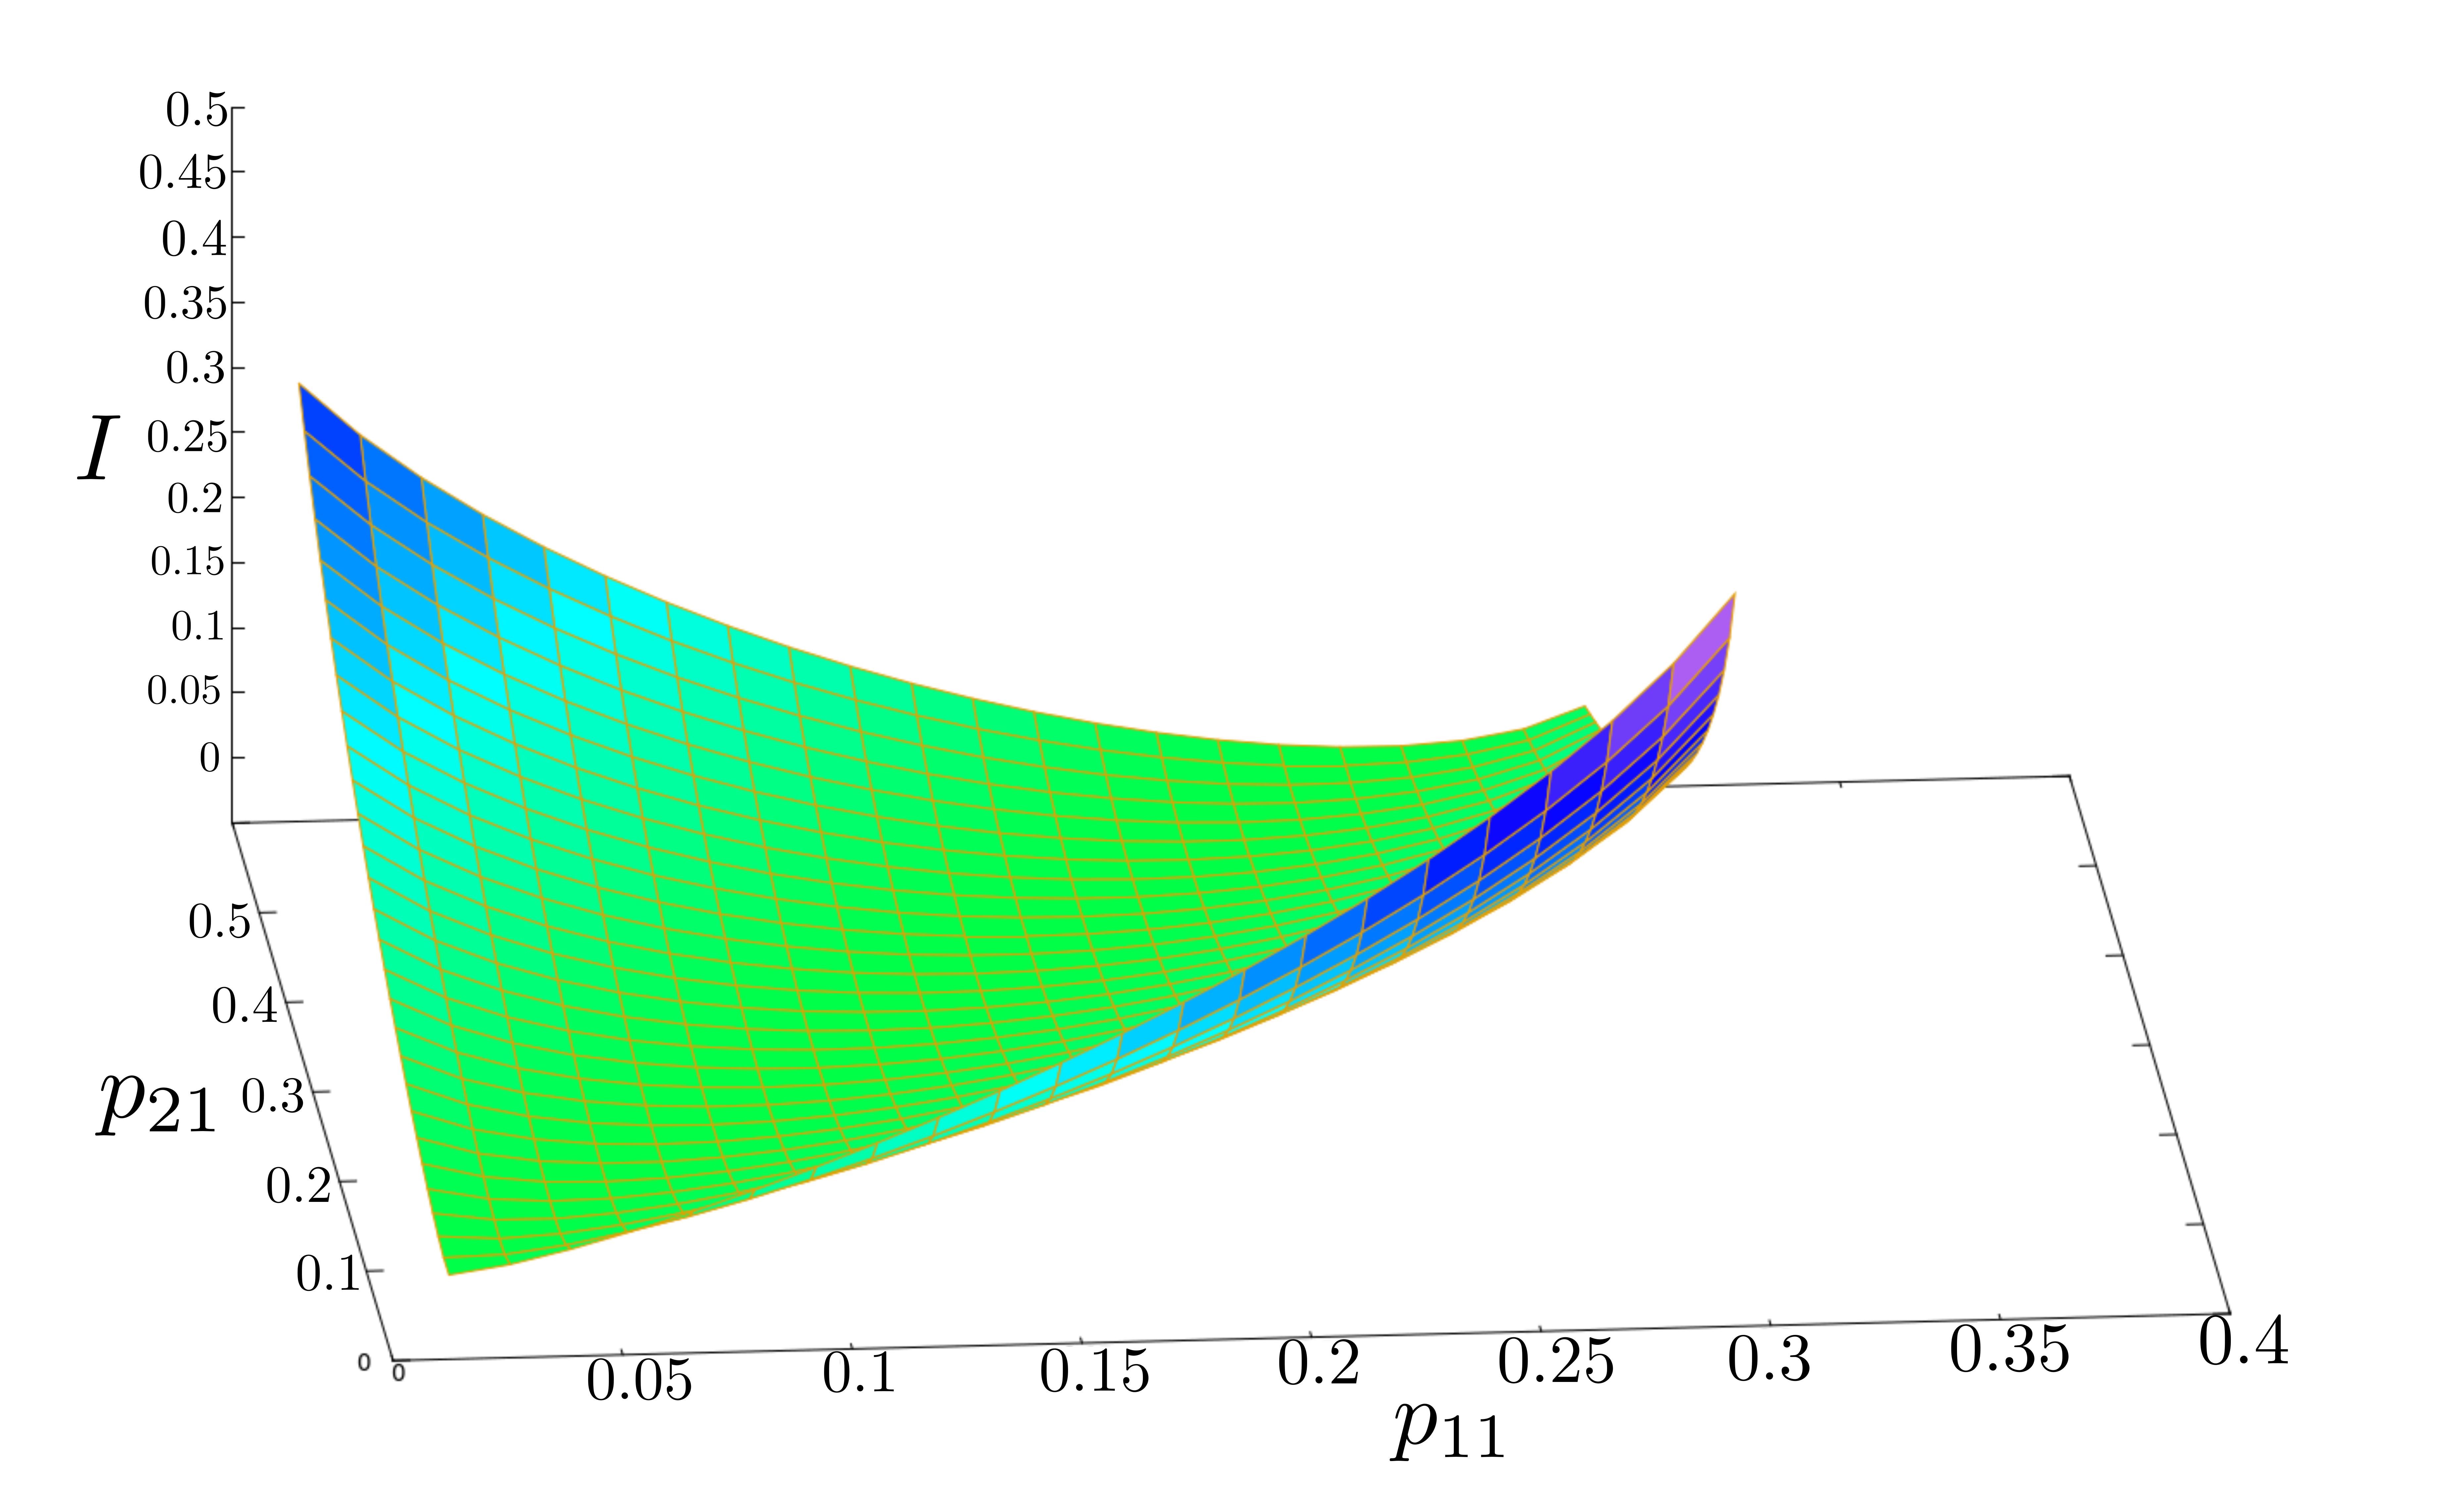
\includegraphics[scale=0.2]{pb/MI_convex.png}
    \caption{Information mutuelle par rapport à la matrice de probabilités}
    \label{fig:mi_convex}
\end{figure}

La convexité semble bien vraie par rapport à $P$, mais on cherche à optimiser les matrices $\Pi_j$. La matrice $P$ comporte les traces de la multiplication $\rho_i \Pi_j$, qui est linéaire par rapport aux coefficients de $\Pi_j$. Si la fonction $I(P)$ est convexe par rapport à $P$, alors elle l'est par rapport aux $\Pi_j$, grace à la linéarité.

Quand on trace la même fonction mais par rapport aux variables $\Pi_{k_{ij}}$, en se fixant dans un espace 2 dimensions, on s'apperçoit que la fonction n'est pas correctement définie sur les bords. Ceci est dû au fait que $x\log(x)$ n'est pas définit pour $x < 0$, ce qui fausse ou bloque les calculs, suivant l'implémentation. Le détail de notre implémentation est expliqué en \ref{fig:xlog}. % TODO: change this to subsubsection reference !

\medbreak

\section{Formulation des contraintes}

La définition du problème permet de résoudre notament les cas immédiats des opérateurs de densité orthogonaux, mais la résolution devient très lente lorsqu'on passe à d'autres cas non orthogonaux. On rajoute des conditions au problème pour accélérer la résolution.

Le premier élément à simplifier est l'expression de l'entropie marginale de $X=\rho_i$. En effet, nous l'avons exprimé en fonction de la trace de la multiplication matricielle, mais on peut reprendre la définition donnée lors du cas classique qui dit que $ H(X) = -\displaystyle \sum_{x \in X} p(x) \log(p(x))$. Le problème nous indique que nous connaissons les probabilités préalables des états d'entrée, on peut donc directement exprimer cette entropie en fonction de ces données et donc sans les variables de sortie $\Pi_i$.

Ensuite, on sait que les opérateurs de mesure se somment à l'identité. Cela signifie d'une part qu'on peut passer d'un problème à $m$ matrices à un problème à $m-1$ matrices pour $m \geq 2$. Les matrices étant carrées de dimension $n$, on passe de $m \times n^2$ variables à $(m - 1) \times n^2$ variables, ce qui est non négligeable.

De plus, le problème et les contraintes sont symmétriques, on peut intervertir les $\Pi_j$ sans influencer le résultat de la fonction coût. Cela nous permet de couper le problème au moins en deux pour réduire à nouveau le temps de calcul. Du fait de la somme à l'identité, on peut ajouter en contrainte que $\Pi_{1_{1, 1}} \leq \frac{1}{m}$ pour $m$ opérateurs de mesure, puis $\Pi_{2_{1, 1}} \leq \frac{1}{m-1}$, etc.

Enfin, pour rappel, les opérateurs de mesure sont des opérateurs densité, qui ne sont pas necessairement purs. Pour qu'ils soient purs, il faudrait entre autre que $\tr(\Pi_i) = 1$. On peut considérer qu'on restreint le problème à un cas purs, et dans ce cas rajouter la contrainte que la somme des éléments diagonaux des opérateurs de mesure doit sommer à 1. Cela permet soit de retirer une variable par matrice densité au problème, en l'exprimant par $x_{n+1} = 1 - \displaystyle \sum_{i}^{n} x_i$ avec les $x_i$ éléments diagonaux de l'opérateur densité, ce qui nécessite une reformulation du problème, soit l'ajout de la contrainte.

\medbreak

\section{Résolution avec \texttt{ibex}}

Pour la résolution de ce problème, utilisons la librairie \texttt{ibex} permettant de faire du calcul par intervale, et possède entre autres un outil d'optimisation, \texttt{ibexopt}. Le problème est formulé avec un langage dédié, \texttt{minibex}. Nous avons eu besoin de définir un opérateur additionnel à ceux présents, l'opérateur \texttt{xlog} permettant d'effectuer l'opération $x \times \log(x)$ en redéfinissant $0 \times \log(0) = 0$ pour que les intervalles ne tombent pas à l'infiniquand ils contiennent 0. De plus, \texttt{minibex} ne considère que des problèmes de minimisation, on ré-écrit le problème en prenant la fonction coût opposée : $\max f(x) \Leftrightarrow \min -f(x)$.
\medbreak
Le premier test effectué est sur le cas de deux états d'entrée $\ket{\psi_1} = \ket{0}$ et $\ket{\psi_2} = \ket{1}$ ayant pour probabilité respective $p_1 = 0.1$ et $p_2 = 0.9$. Le résultat théorique est connu: les états étant orthogonaux, on doit obtenir les opérateurs de mesure égaux aux opérateurs densité d'entrée. On obtient bien avec \texttt{ibex} les opérateurs suivant:

$\Pi_1 = \begin{bmatrix} 0 & 0 \\ 0 & 1\end{bmatrix} , \quad \Pi_2 = \begin{bmatrix} 1 & 0 \\ 0 & 0\end{bmatrix},$

qui correspondent bien à deux opérateurs de mesure orthogonaux. Dans ce cas, l'information mutuelle est comprise dans l'intervalle $I(\rho, \Pi) \in [0.3250, 0.3254]$, avec un temps de calcul de 8.6 millisecondes.
\medbreak
Le deuxième cas qu'on peut présenter est le suivant: $\ket{\psi_1} = \ket{0}$ et $\ket{\psi_1} = \ket{+}$ avec comme probabilité respectives $p_1 = 0.1$ et $p_2 = 0.9$. Le résultat théorique n'est pas donné, et on obtient avec \texttt{ibex} le résultat suivant:

$\Pi_1 = \begin{bmatrix} 0.445 & 0.497 \\ 0.497 & 0.555\end{bmatrix} , \quad \Pi_2 = \begin{bmatrix} 0.555 & -0.497 \\ -0.497 & 0.445\end{bmatrix},$

avec une information mutuelle comprise dans l'intervalle $I(\rho, \Pi) \in [0.1348, 0.1349]$, et un temps de calcul de 0.79 secondes.

% On voit bien avec ces deux exemples l'augmentation radicale du temps de calcul quand on passe d'un problème simple, même orthogonal, à un problème plus compliqué.

En revanche, ibex ralentit fortement dès qu'on sort des cas simples présentés si-dessus, et notament quand on retire la restriction des opérateurs de mesure à des opérateurs densité purs (de trace unitaire). Deux éléments importants sont à l'origine du problème. Tout d'abord, en analysant l'utilisation des ressources cpu lors de la résolution d'un problème, on voit qu'un seul thread est utilisé par \texttt{ibexopt}. Les algorithmes d'optimisation peuvent être parallélisés, et dans le cas de processeurs à plusieurs c\oe urs on pourrait avoir un gain de performance conséquent. Le deuxième élément est en lien avec la convexité de la fonction coût évoqué précédement. On eut alors se limiter aux extremités de la fonction coût pour réduire le nombre de calculs à effectuer. Il faudrait alors implémenter la condition $0 \in [\texttt{grad}]([f])$, ce qui n'est pas prévu de base dans \texttt{ibexopt}.


\section{Exemple}

Prenons le cas de deux états quantiques:

\begin{align}
    \ket{\psi_1} = \begin{bmatrix}\frac{1}{3} \\ \frac{2 \sqrt{2}}{3}\end{bmatrix} , \quad \ket{\psi_2} = \begin{bmatrix}\frac{1}{\sqrt{2}} \\ \frac{1}{\sqrt{2}}\end{bmatrix},
\end{align}
avec les probabilités préalables 
\begin{align}
    p(\ket{\psi_1}) = 0.1, \quad p(\ket{\psi_2}) = 0.9.
\end{align}

Ces deux états peuvent être réécris sous la forme d'opérateurs densité $\rho_1 = \begin{bmatrix}\frac{1}{9} && \frac{2 \sqrt{2}}{9} \\ \frac{2 \sqrt{2}}{9} && \frac{8}{9} \end{bmatrix}$ et $\rho_2 = \begin{bmatrix}\frac{1}{2} && \frac{1}{2} \\ \frac{1}{2} && \frac{1}{2} \end{bmatrix}$.

Le problème est de trouver les deux opérateurs densité optimaux au sens de l'information mutuelle. On considère le problème comme ne possédant pas de termes complexes sur les antidiagonaux, et l'équation \ref{eq:contrainte_somme_id} nous permet de réduire le problème à trois variables seulement $\{a_1, b_1, d_1\}$ :

\begin{align}
    \Pi_1 &= \begin{bmatrix}a_1 && b_1 + ic_1 \\ b_1 - ic_1 && d_1\end{bmatrix} = \begin{bmatrix}a_1 && b_1 \\ b_1 && d_1\end{bmatrix} \\
    \Pi_2 &= I - \Pi_1 = \begin{bmatrix}1 - a_1 && -b_1 \\ -b_1 && 1 - d_1\end{bmatrix}
\end{align}

On pose ensuite les contraintes sur ces variables. Tout d'abord, ces variables sont définies sur ces bornes spécifiques: $a_1 \in [0, 0.5]$, $b_1 \in [-1, 1]$, $d_1 \in [0, 1]$. La détermination de la semi-définition positive passe par les diagnonales et le déterminant strictement positifs, d'une part avec les bornes précédentes et d'autre part avec deux nouvelles contraintes sur les 3 variables.
Le problème s'écrit donc :

\begin{align}
    \max\limits_{a_1, b_1, d_1} I(a_1, b_1, d_1) , \nonumber
\end{align}
tel que :
\begin{align}
    &a_1 \in [0, 0.5] , b_1 \in [-1, 1] , d_1 \in [0, 1] , \nonumber \\
    &a_1 * d_1 - b_1^2 \geq 0 , \nonumber \\
    &(1-a_1) * (1-d_1) - b_1^2 \geq 0. \nonumber
\end{align}

La résolution avec \texttt{ibex} ou avec notre solveur donne les deux opérateurs de mesure suivants: 

\begin{align}
    \Pi_1 = \begin{bmatrix}0.456 && -0.498 \\ -0.498 && 0.544\end{bmatrix}, \quad \Pi_2 = \begin{bmatrix}0.544 && 0.498 \\ 0.498 && 0.456\end{bmatrix},
\end{align}

Avec une information mutuelle $I(a_1, b_1, d_1) = 0.04723$. Notre solveur résout le problème en $6.4$ secondes pour une précision sur $I$ de $1 \times 10^{-5}$, et \texttt{ibexopt} résout en $88.3$ secondes pour une précision sur $I$ de $4\times 10^{-5}$.
